%!TEX root = practicum2.tex
\Cref{alg:percolation} presents our iterative growth process, the method \FuncSty{percolation} expects three arguments \t{N}, \t{probability} and \t{mask}. Given the size parameter \t{N}, the grid used for the percolation is $(N + 1) \times (N + 1)$, since this causes the grid to have an uneven number of rows and columns its center is always clearly defined as $(N, N)$. The parameter $p \in [0, 1]$ is the probability that a given site in the cluster becomes occupied. The \t{mask} is a binary matrix with $r$ rows and $c$ columns that determines the used connectivity, until \cref{ss:exp:connectivity} we only consider four-connected clusters, which use the mask presented in \cref{fig:exp:connectivity:fourMask}.

\begin{figure*}
	\centering	
	\begin{subfigure}{0.27\textwidth}
		\centering
		
\includegraphics[width=0.9\textwidth]{./img/fancy_cluster_N20_p3_rng_8}
		\caption{$N = 20$ and $p = 0.3$}
		\label{fig:method:fin_inf:finiteSmall}
	\end{subfigure}
	\begin{subfigure}{0.27\textwidth}
		\centering
		
\includegraphics[width=0.9\textwidth]{./img/fancy_cluster_N20_p5_rng_8}
		\caption{$N = 20$ and $p = 0.5$}
		\label{fig:method:fin_inf:finiteLarge}
	\end{subfigure}	
	\begin{subfigure}{0.27\textwidth}
		\centering
		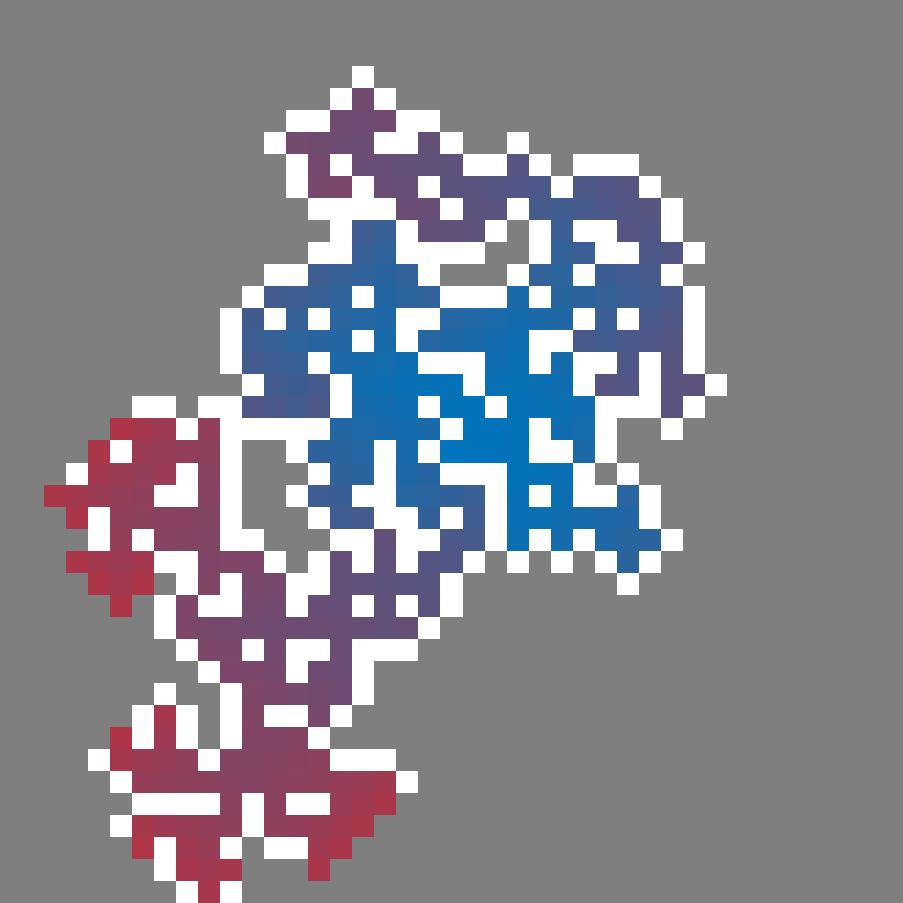
\includegraphics[width=0.9\textwidth]{./img/fancy_cluster_N20_p6_rng_5}
		\caption{$N = 20$ and $p = 0.6$}
		\label{fig:method:fin_inf:infinite}
	\end{subfigure}		
	\caption{Examples of \subref{fig:method:fin_inf:finiteSmall} a small finite cluster, \subref{fig:method:fin_inf:finiteLarge} a larger finite cluster and \subref{fig:method:fin_inf:infinite} a percolating cluster using four-connected neighbours. The colours of the elements in the cluster indicate when that point was added to the cluster, the `colder' the color the earlier in the percolation it was added to the cluster. White cells are empty and gray cells are undetermined. }
	\label{fig:method:fin_inf}
\end{figure*}

\begin{algorithm}[t]
	\setstretch{1.2}
	\SetAlgoShortEnd
	\DontPrintSemicolon
	\SetKwInOut{Input}{input}\SetKwInOut{Output}{output}
	\Input{$N$ size\\
		$p$ probability\\
		$mask$ $r \times c$ binary matrix.}
	\Output{$grid$ $(N + 1) \times (N + 1)$ matrix}
	\BlankLine

	$center$ := ($N + 1$, $N + 1$)\; 
	\FuncSty{push($queue$, $center$)}\; 
	$grid$ := \FuncSty{initGrid($N$, $N$)}\; 

	\While{not \FuncSty{isEmpty($queue$)}}{
		$site$ = \FuncSty{pop($queue$)}\; 
		$sites$ = \FuncSty{grow}($grid$, $site$, $mask$, $p$)\; 
		\If{onBorder(site)}{
			\KwSty{break}
		} 
		\FuncSty{push($queue$, $sites$)}\; 
	}\; 
	\caption{\FuncSty{percolation}$(mask, N, p)$\label{alg:percolation}}
\end{algorithm}

% Initialisation
Initially the only site we have to consider is the center site, which is consquently the only site in the queue at the first iteration.

% Iteratie
Each iteration we pop the next \t{site} from the queue. We grow this point, using the function \t{grow}. This method considers all neighbors that are connected to \t{site} according to \t{mask}. For each of these neighbors we determine the value $z$, which is randomly sampled from an uniform distribution with the range $[0,1]$. If $z \leq p$ we mark the neighbor site as occupied, otherwise it is marked empty. The method \t{grow} returns the neighbor sites that are occupied, these are added to the queue, as these sites are should also be allowed to grow. 

% Stop conditions
The growth of the clusters stops if it cannot grow anymore or if it has reached one of the borders of the grid. In the first case the cluster is finite, which means that all neighbor sites of the cluster, according to the connectivity defined by the \t{mask}, are marked as empty. In \cref{alg:percolation} we test for this condition via the guard of the loop; if the queue is empty there are no more neighbors to consider, consequently the cluster must be finite. 

A percolating cluster is a cluster that has reached the border of the grid, i.e. if there is a occupied site with row or column number $1$ or $2N + 1$. We test for this condition with the method \t{onBorder}. It should be noted that we only check if a site is on the border of the grid after we have already grown the site. 

\Cref{fig:method:fin_inf} presents three clusters grown with the algorithm. We can clearly see that the finite clusters are completely surround by a white border, which indicates that these sites are empty. The illustration of the percolation cluster, \cref{fig:method:fin_inf:infinite}, shows that although there are still sites that can grow indicate by the lack of white neighbors, there is one site on the border near the bottom left corner of the image that has stopped the percolation. 
